\documentclass[11pt]{extarticle}
\usepackage[utf8]{inputenc}
\usepackage{cite, authblk, mdframed}
\usepackage[margin=1in]{geometry}
\usepackage{graphicx}

\title{Project: Midterm Report}
\author[1]{Evan Matthews}
\author[1]{Vikram Ramavarapu}
\author[1]{Krishnaveni Unnikrishnan}
\affil[1]{CS 412 Group G6}
\date{November 6th, 2024}

\newcommand{\todo}{\textcolor{red}{TODO:}~}

\begin{document}

\maketitle

\pagebreak

% \section{Title} 
% starting with group id, please also include names of group members

\section{Abstract}
\todo summarizing the project\cite{Pettorruso2020-qt,Cash2012-rb,Aboujaoude2010-mc,Restrepo2020-pb}.

\begin{mdframed}
\end{mdframed}

\section{Introduction}

The internet has become an integral part of our daily lives, with people of all ages spending a significant amount of time online. 
This trend has given rise to concerns about the potential impacts of excessive internet use, particularly on children and teens.
Problematic Internet Use (PIU) is a condition characterized by excessive or poorly controlled preoccupations, urges, or behaviors regarding computer use and internet access that lead to impairment or distress \cite{Pettorruso2020-qt}. 
PIU has been associated with a range of mental health issues, including depression, anxiety, and impulsivity \cite{Cash2012-rb}.
As such, identifying early signs of PIU in children and teens is crucial for prevention and intervention.
In this project, we aim to predict early signs of PIU in children and teens using machine learning techniques, leveraging data from the Child Mind Institute's Healthy Brain Network.
The project plan consists of three phases: data preprocessing, initial model evaluation, and fine-feature reevaluation.
We will submit our work to the Child Mind Institute's (CMI) Kaggle competition on PIU prediction, and we also aim to publish our results as a paper should they outperform competition expectations.


\section{Motivation} 

\begin{mdframed}
    With the rise of machine learning and pattern prediction models, the ability to analyze and predict upon more complex data and parameters becomes much more approachable.
    Likewise, child development is a multi-facted situation in which parenting and environmental factors can lead to an incredibly high number of outcomes.
    This field has had great strides in classical research, but a more modern approach could lead to significant development in the success of future generations.
    Additionally, predictions against an extensive number of possible outcomes like this represents a current roadblock in machine learning- that is, how modern predictive models can adapt to an ever-increasing set of parameters and decreasing set of training data.
    Finally, child psychology is interested in recognizing patterns in early behavior in order to reduce the impact of harmful effects from a child's environment.
\end{mdframed}

\section{Related work} 

\begin{mdframed}
    Research on Problematic Internet Use (PIU) has gained significant attention due to its increasing prevalence and association with various psychological and behavioral issues. Early investigations into PIU highlighted its similarities with substance use disorders, impulse control disorders, and obsessive-compulsive disorder.
    
    Studies have revealed concerning prevalence rates between 1.5\% and 8.2\% in the United States and Europe, emphasizing the growing social impact of this condition. 
    The relationship between PIU and psychiatric disorders has been extensively documented, with research showing significant associations with depressive disorders and attention-deficit/hyperactivity disorder (ADHD). 
    A notable study found that individuals with PIU were more than twice as likely to have depressive disorders $(aOR = 2.43)$, and showed increased likelihood of having ADHD combined presentation $(aOR = 1.91)$ and Autism Spectrum Disorder $(aOR = 2.24)$.
    
    Recent investigations have focused on understanding the personality profiles and emotional factors contributing to PIU. Research has identified specific personality traits associated with PIU, including lower scores in novelty seeking, harm avoidance, and reward dependence. 
    Additionally, emotional dysregulation has emerged as a significant factor, with studies suggesting that PIU may serve as a behavioral mechanism for escaping negative affects.
    
    Treatment approaches for PIU have primarily centered on addressing comorbid conditions, with cognitive behavioral therapy and selective serotonin reuptake inhibitors showing promise as potential interventions.
    However, researchers emphasize that detailed treatment guidelines require further investigation, particularly given the complex interplay between PIU and various psychological disorders.
    
    The field continues to evolve, with ongoing debates about diagnostic criteria and classification. While the Internet's positive impact on well-being is widely acknowledged, the pathological aspects of its use remain understudied, particularly regarding subtle psychological changes such as online disinhibition. 
    This highlights the need for additional research into the pathophysiology, epidemiology, natural course, and treatment of PIU to develop more effective intervention strategies.
\end{mdframed}

\section{scope}

    Given that the original scope of the project was accepted, we are pressing forward with this plan with no significant changes.
    The most crucial critique provided- that the validation plan and evaluation metric were not clear- are likewise addressed in the methodology section.

\section{Methodology} 
% \todo what you are doing / planning to do from a data mining perspective. 
% This can include any exploratory or statistical data analysis, visualization, efficient data storage/compression, fitting predictive models, clustering, pattern mining, etc.  
% If you are doing / planning to do a comparative study, discuss the methods you are considering, including any methods being used as baselines.  
% Please include a clear evaluation plan, including train-val-test splits, cross-validation, hyper-parameter tuning, and explain clearly how you will do these. 
% You have to highlight alignment of the project with the course clearly, especially if you have received feedback on concerns regarding limited alignment with the course. 

Data for this project has two components: cross-sectional, and time-series. The cross-sectional data is per participant and contains fields described in the following table (etcetc).
Each time-series dataset is per participant and each entry of the dataset represents the status of the participant's heartrate monitor at a given point in time.

The project will be divided into three phases: data preprocessing, initial model evaluation, and fine-feature reevaluation.
The data preprocessing phase entails dropping fields where survey responses are recorded and are then used to compute the SII, as our model's intention is to compute SII directly from the other metrics.
Missing values in the data are filled using iterative imputation, and the missing SII values are filled in using K-Nearest Neighbors (k=5).

Multiple models will be evaluated on the cross-sectional data: Random Forest, XGBoost, SVM, and a feed forward neural network. After this, a sequential model, evaluated amongst transformers or auto-encoders, will be trained on the time-series data. The sequential model will allow us to compute an embedding of the time-series data, which will be used as an additional feature in the cross-sectional model.
The final model will be an ensemble of the cross-sectional and sequential models, with the sequential model's embedding as an additional feature in the cross-sectional model. The classifier model will be retrained on the concatenated dataset, to predict the SII.

\section{(Current / Preliminary) Results} 
\todo what you have so far in terms of initial results and analysis of initial results. Please see comment on figures/tables above, especially the fact that good captions go a long way to making things readable.

\begin{figure}[h]
    \centering
    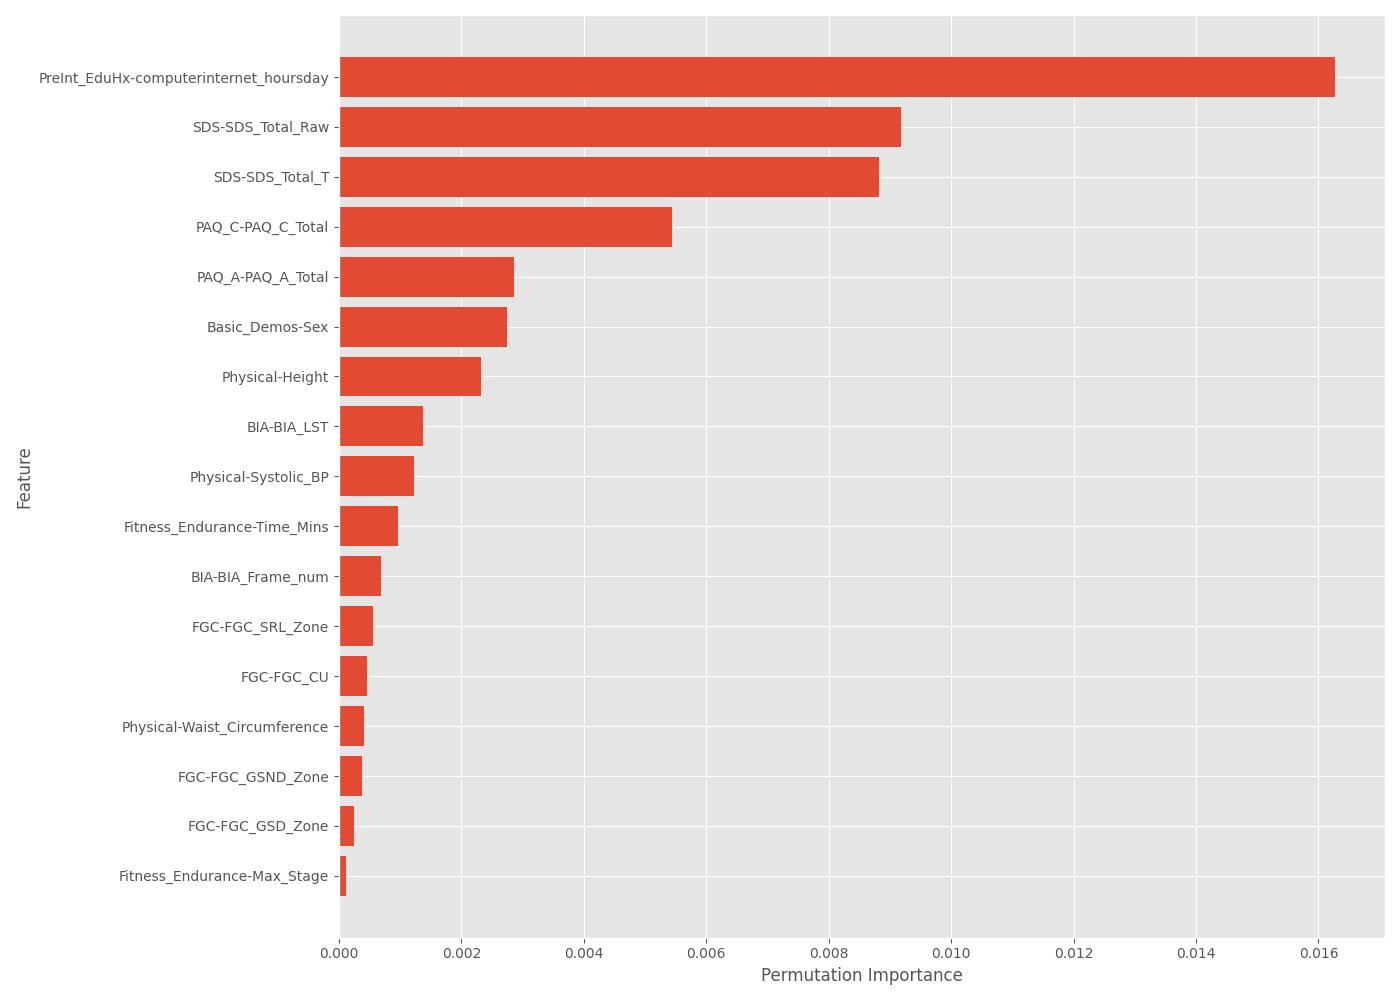
\includegraphics[scale=0.4]{"./feature_importance.jpg"}
    \caption{Features plotted in order of importance, ascending.}
\end{figure}

\begin{mdframed}
    Add results here
\end{mdframed}

\section{Plan of Work} 
\todo what are the next steps before the final report. Please be as precise as possible. Note that you will have about a month to finish the project, so make suitably calibrated plans, e.g., do not over/under promise.

\begin{mdframed}
    Add plan of work here
\end{mdframed}

\section{Conclusions, discussions}

\begin{mdframed}
    add conclusions here
\end{mdframed}

\bibliographystyle{plain}
\bibliography{bibliography}

\end{document}